\documentclass{beamer}	
\mode<presentation>
 
\usepackage{pdfpages}
\usepackage{fancyvrb}
\usepackage{chemarr}

\usepackage{amsmath}		%% mathematics typesetting
\usepackage{amssymb}
 
\usepackage{ulem}

\usepackage{booktabs}

\usepackage{siunitx} %% tpyeset SI units

\usepackage{CJKutf8} %% typeset Chinese characters

\usepackage{pdfpages}

% Color and Theme. Can be changed. However, this one's quite nice.
\usetheme{Madrid}
\definecolor{theme}{rgb}{0.84,0,0.21}
\usecolortheme[named=theme]{structure}


%%  Title information
\title[Literatur-Recherche]{Wie erfahre ich von medizinischer Forschung? \\
Einführung in die Literatur-Recherche}
\author[melanie.stefan@medicalschool-berlin.de]{M14 Wissenschaftliches Arbeiten}
\institute[]{Prof. Melanie Stefan - melanie.stefan@medicalschool-berlin.de}
\date{WiSe 2023/24}
 

% Table of contents to pop up at the beginning of each section
\AtBeginSection[]
{
  \begin{frame}<beamer>
    \frametitle{Outline}
    \tableofcontents[currentsection,currentsubsection]
  \end{frame}
}
 
\beamertemplatenavigationsymbolsempty

\begin{document}
 
 
 
{ \usebackgroundtemplate{
\includegraphics[width=1.2\paperwidth]{MSB_Titelseite.pdf}} 
\begin{frame}

 \maketitle 

$\,$\\[6cm] 


\end{frame} 
}



 
%% Hook
\begin{frame}{Sie wissen, wie man wissenschaftliche Literatur liest\dots}

\begin{center}
    \includegraphics[width=\textwidth]{annie-spratt-CV3nkG7XIwg-unsplash.jpg}
\end{center}

    
\end{frame}


\begin{frame}{Aber wo finden?}

\begin{center}
    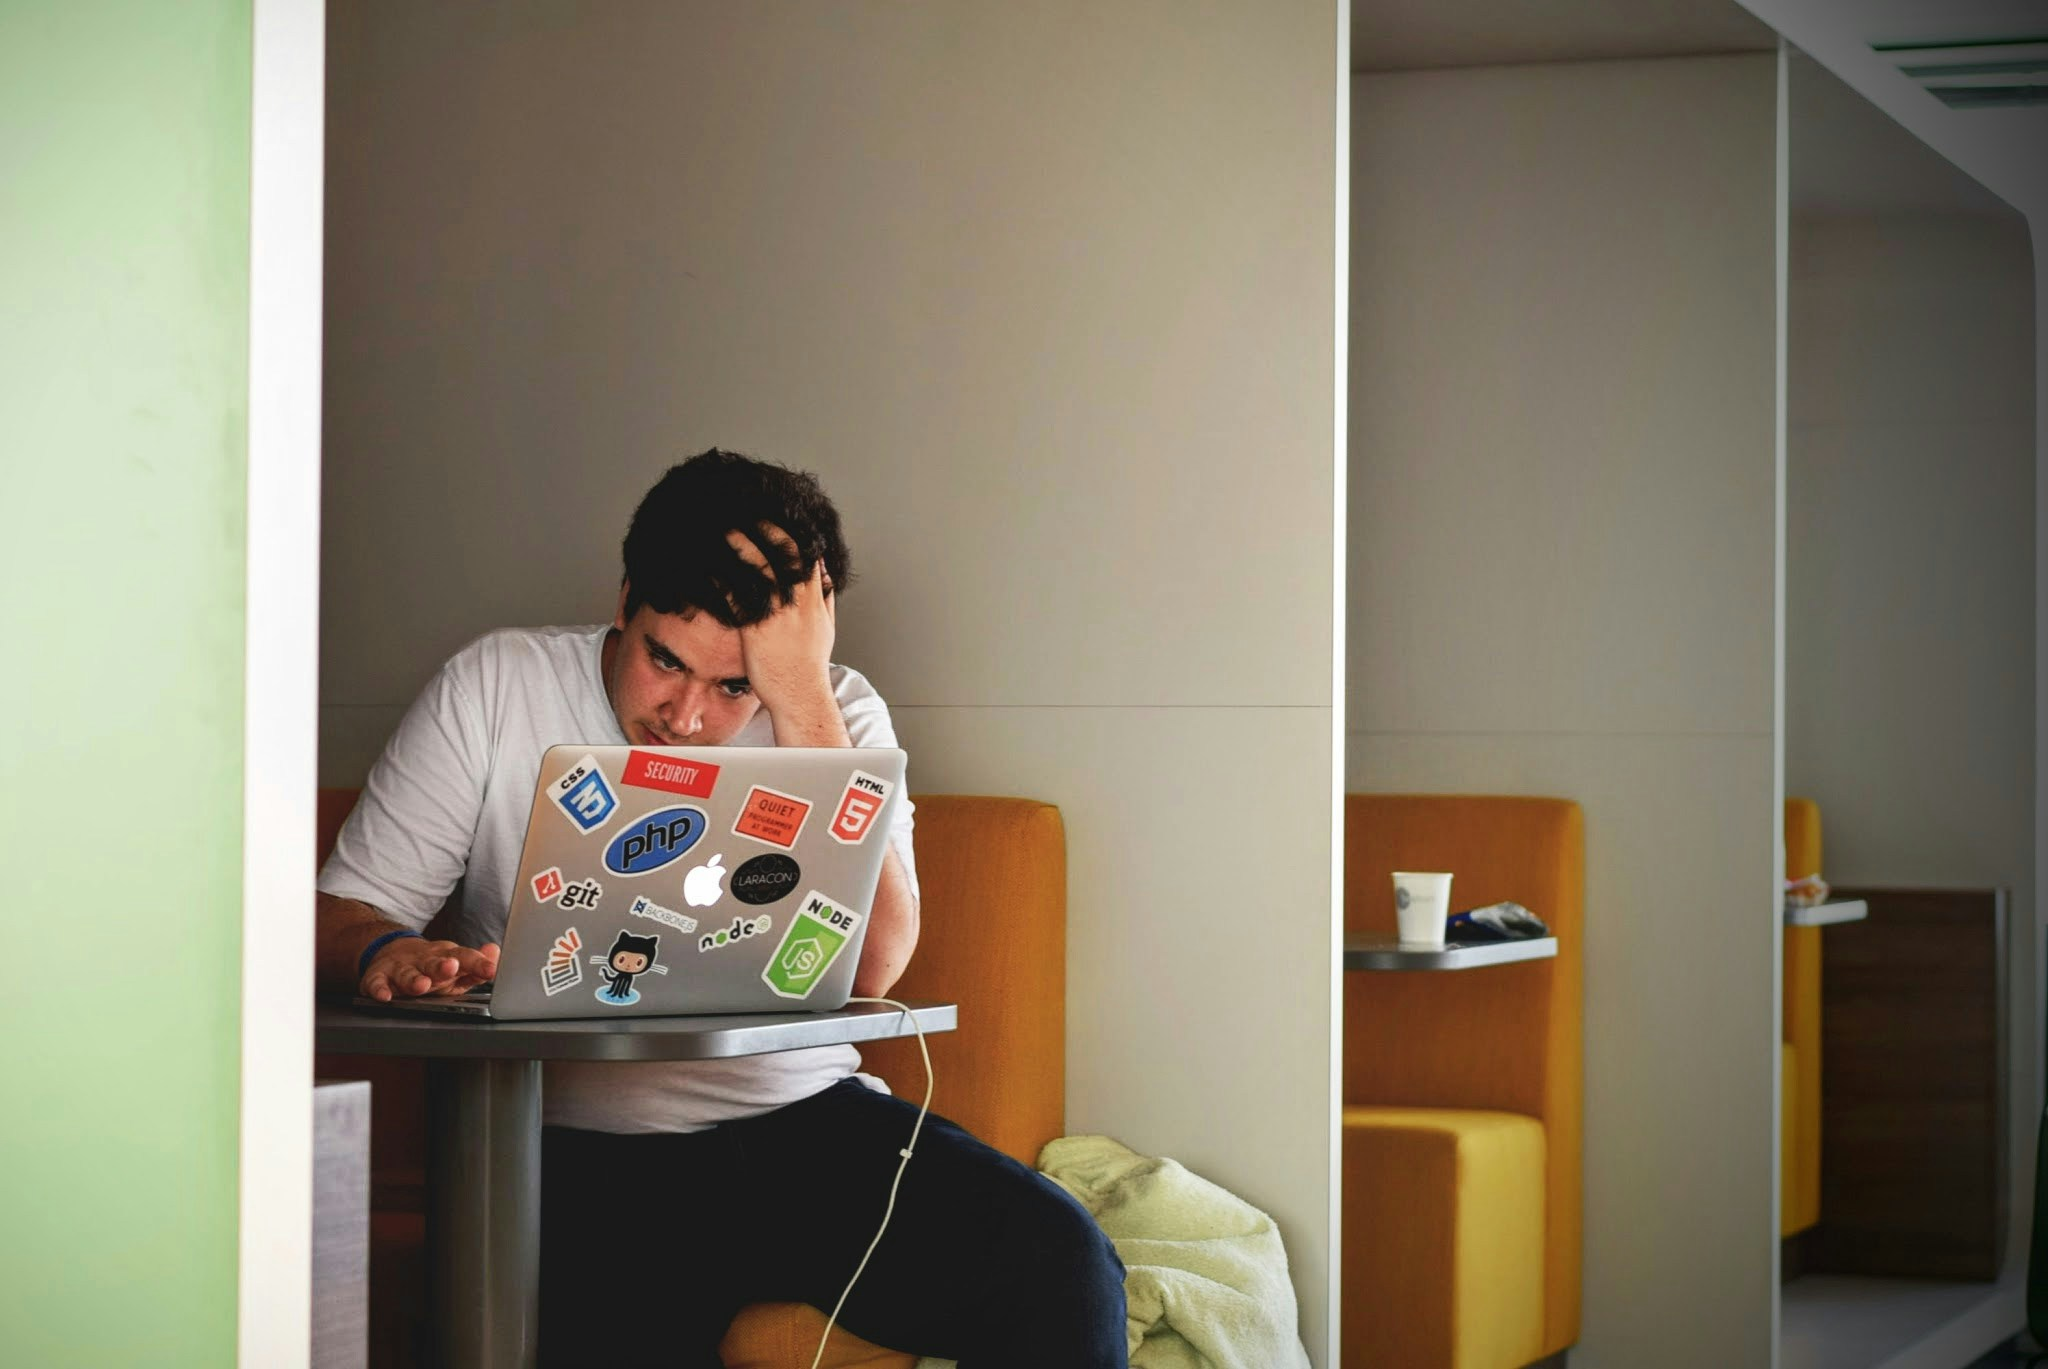
\includegraphics[width=\textwidth]{tim-gouw-1K9T5YiZ2WU-unsplash.jpg}
\end{center}

    
\end{frame}


%% TLIA
\begin{frame}
\frametitle{In dieser Vorlesung geht es um \dots}

\dots wissenschaftliche Information, wie sie geteilt wird, und wie wir sie gezielt suchen und finden können.

\begin{center}
    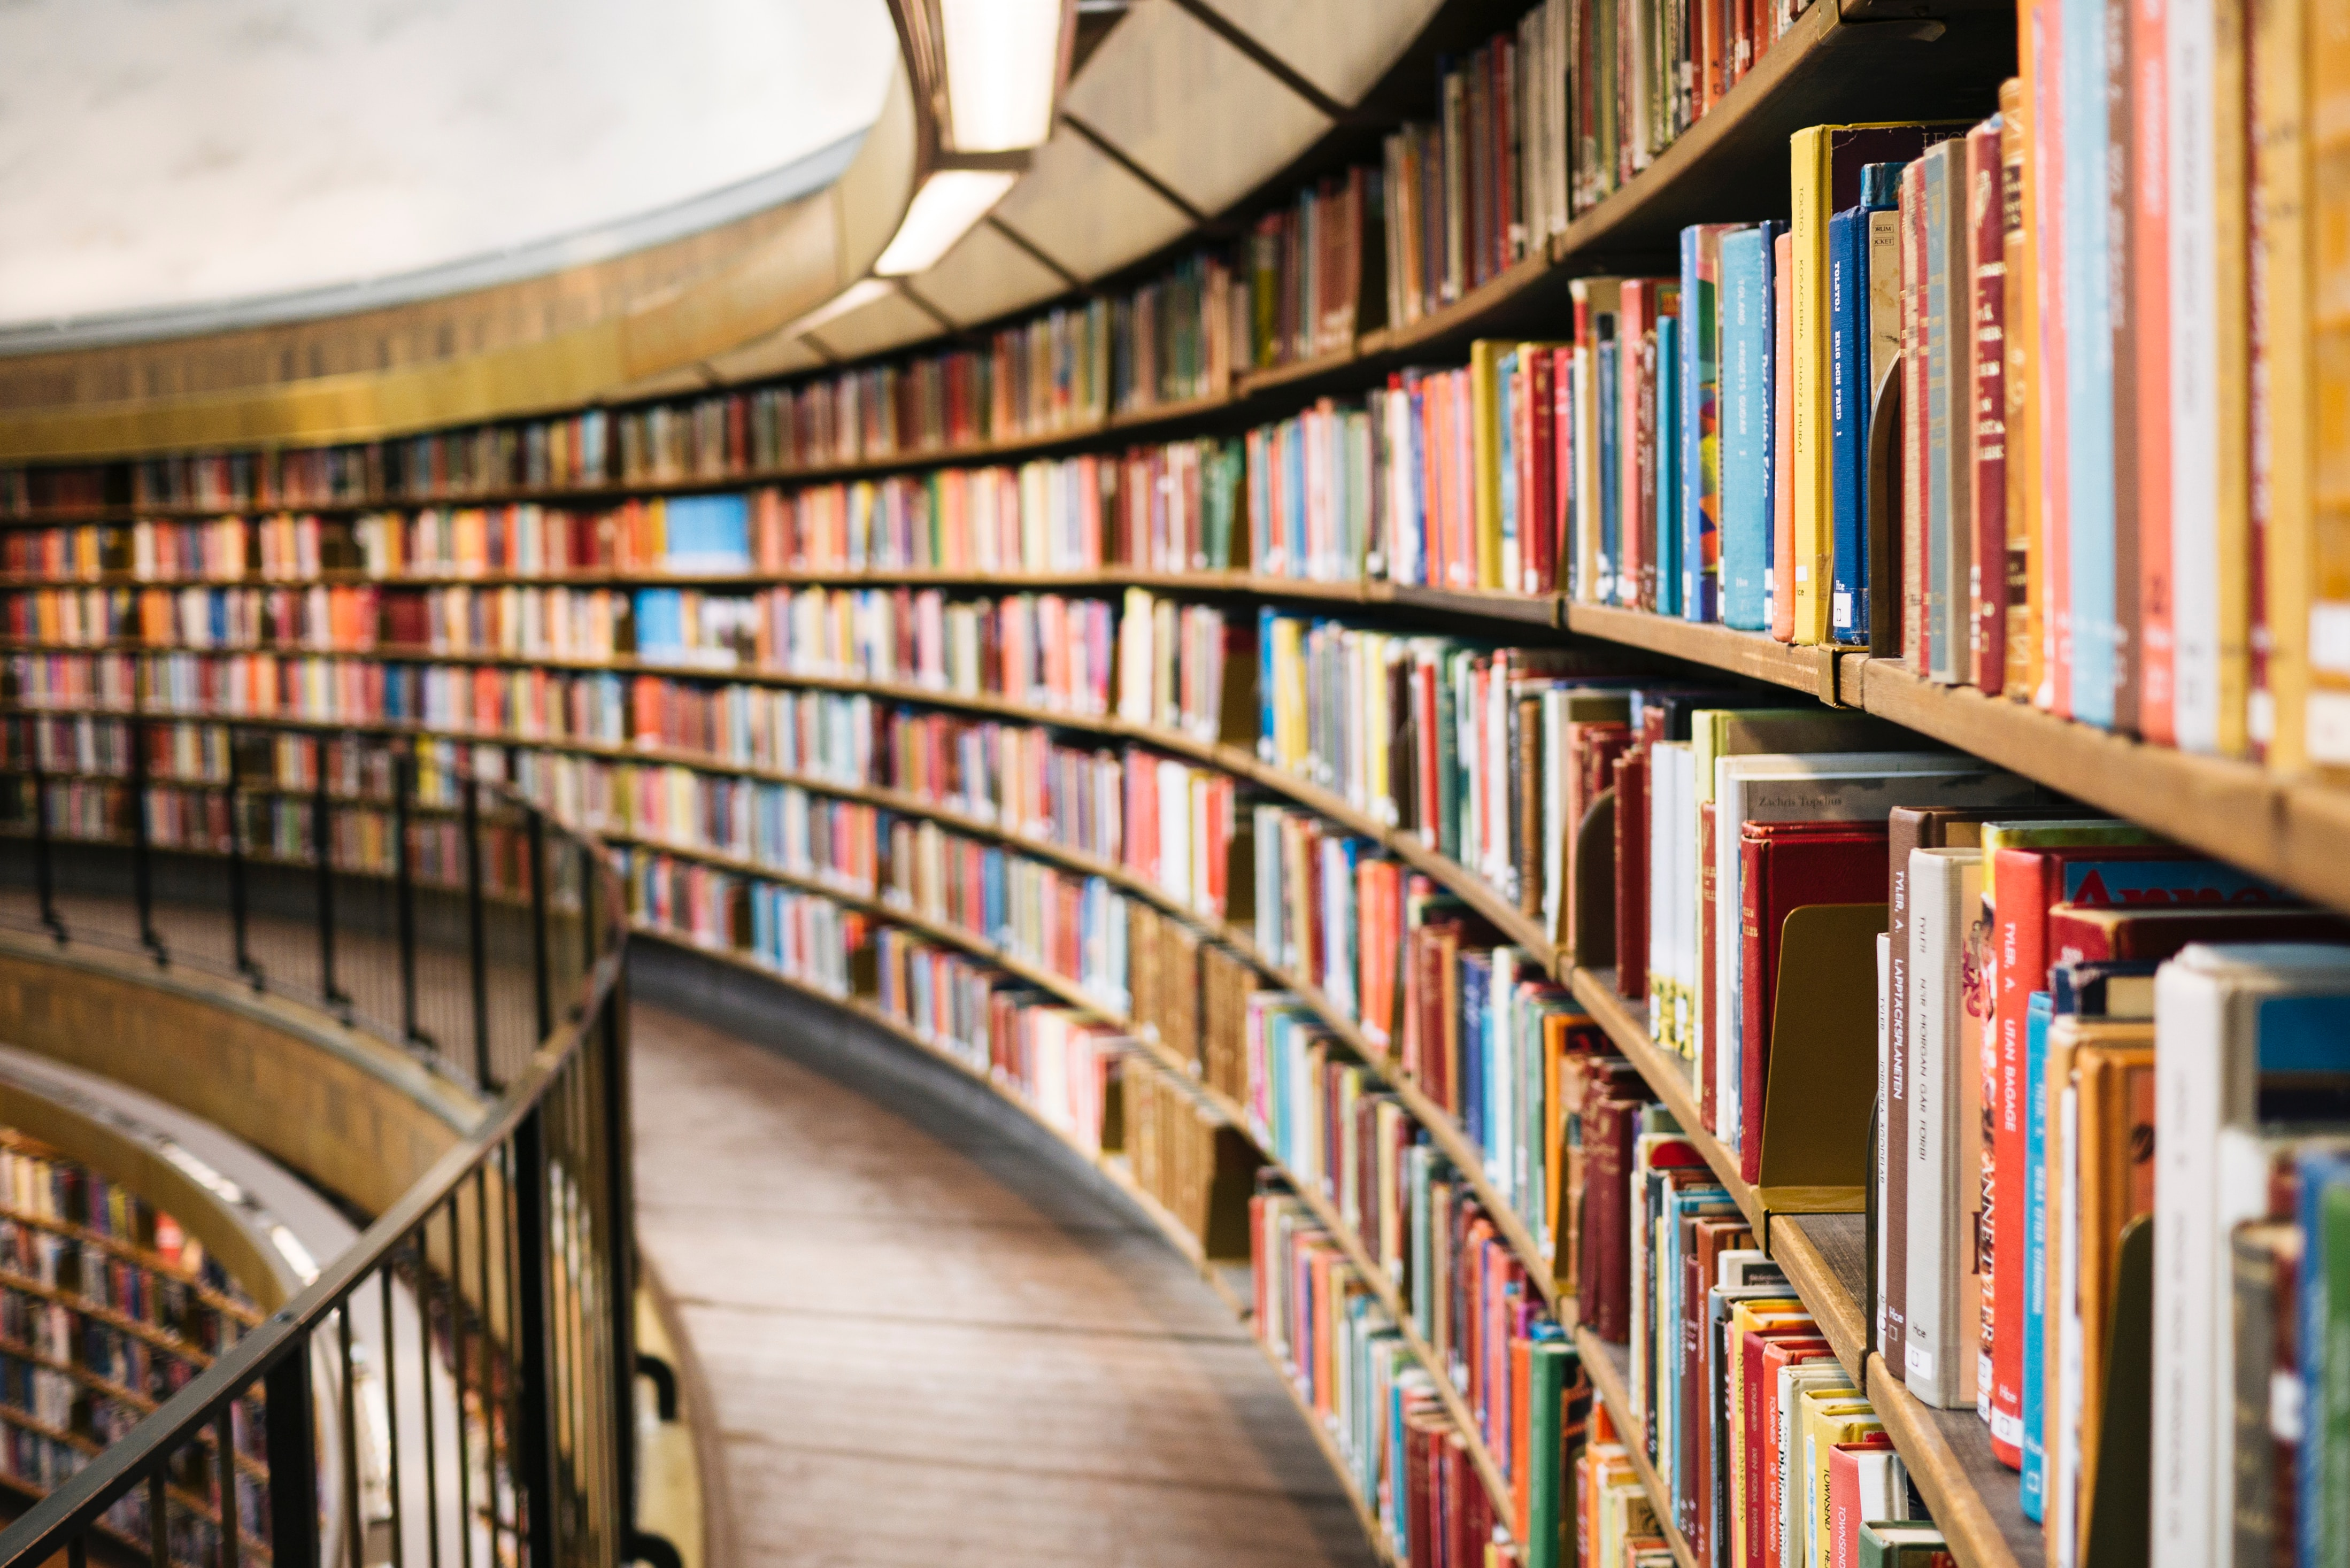
\includegraphics[width=0.7\textwidth]{susan-q-yin-2JIvboGLeho-unsplash.jpg}
\end{center}


 
\end{frame}



%% Learning Objectives

\begin{frame}

\frametitle{Nach dieser Vorlesung sollten Sie \dots}


\begin{itemize}
\item
Wissen, was die Bibliothek der MSB zu bieten hat
\item 
Medizinisch relevante Information finden
\item 
Medizinische Informationsquellen kritisch bewerten
\item 
Mehrere Wege kennen, um Zugang zu Büchern zu bekommen
\item 
Erklären, wie medizinische Forschungsergebnisse kommuniziert und publiziert werden
\item 
Verschiedene Datenbanken und Tools zur Literaturrecherche kennen und deren Vor- und Nachteile aufzählen
\item 
Strategien der Literaturrecherche aufzählen und vergleichen
\item 
Gezielt nach Literatur suchen
\item 
MeSH Terms und Boolean Operators bei der Literaturrecherche verwenden
\item 
Gefundene Literatur sammeln und verwalten
\end{itemize}

\end{frame}

%% Main Body


\section{Woher bekomme ich medizinische Information? }

\begin{frame}{Was sind Ihre Quellen, wenn Sie Information über ein medizinisches Thema brauchen?}



\end{frame}

% - Bib
% - Via Medici etc.
% - Wikipedia
% - Bücher
% - online portale
% -chatgpt

% %% Online Quellen
%  \begin{frame}
% \frametitle{Weitere Quellen}

% \begin{itemize}
% \item 
% Via Medici (nicht immer korrekt!)
% \item
% Formelsammlungen (am besten selber zusammenstellen)
% \item 
% Wikipedia: oft guter Überblick und nützliche weiterführende Quellen. Ersetzt aber nicht das Lehrbuch. 
% \end{itemize}


% \end{frame}


%  \begin{frame}
% \frametitle{Was ist mit ChatGPT?}

% \pause 

% \includegraphics[width=0.9\textwidth]{chatgpt_geographie_frage.png}

% \vfill
% \end{frame}


%  \begin{frame}
% \frametitle{ChatGPT ist eine Sprachmaschine, keine Faktenmaschine!}


% \includegraphics[width=0.9\textwidth]{chatgpt_geographie.png}

% \end{frame}


\section{Wie wird medizinische Forschung kommuniziert und publiziert?}

\section{Wie kann ich wissenschaftliche Literatur finden?}


%% pubmed google scholar biorxiv scihub


\section{Was mache ich mit der gefundenen Literatur?}




%% Review


\begin{frame}

\frametitle{Jetzt* sollten Sie \dots}


\begin{itemize}
\item
Wissen, was die Bibliothek der MSB zu bieten hat
\item 
Medizinisch relevante Information finden
\item 
Medizinische Informationsquellen kritisch bewerten
\item 
Mehrere Wege kennen, um Zugang zu Büchern zu bekommen
\item 
Erklären, wie medizinische Forschungsergebnisse kommuniziert und publiziert werden
\item 
Verschiedene Datenbanken und Tools zur Literaturrecherche kennen und deren Vor- und Nachteile aufzählen
\item 
Strategien der Literaturrecherche aufzählen und vergleichen
\item 
Gezielt nach Literatur suchen
\item 
MeSH Terms und Boolean Operators bei der Literaturrecherche verwenden
\item 
Gefundene Literatur sammeln und verwalten
\end{itemize}

\end{frame}


%% Bildnachweis
\begin{frame}
\frametitle{Bildnachweis}


\begin{tiny}
 
\begin{itemize}

\item 
Bibliothek. Photo by \href{https://unsplash.com/@syinq?utm_content=creditCopyText&utm_medium=referral&utm_source=unsplash}{Susan Q Yin} on \href{https://unsplash.com/photos/books-on-brown-wooden-shelf-2JIvboGLeho?utm_content=creditCopyText&utm_medium=referral&utm_source=unsplash}{Unsplash}
  

\item 
Frau sitzt am Laptop und konzentriert sich. Photo by \href{https://unsplash.com/@anniespratt?utm_content=creditCopyText&utm_medium=referral&utm_source=unsplash}{Annie Spratt} on \href{https://unsplash.com/photos/woman-in-black-long-sleeve-shirt-using-macbook-air-on-brown-wooden-table-CV3nkG7XIwg?utm_content=creditCopyText&utm_medium=referral&utm_source=unsplash}{Unsplash}
  

  
\item
Logo der MSB. MSB Medical School Berlin, Public Domain, via Wikimedia Commons

\item 
Mann sitzt am Laptop und rauft sich die Haare. Photo by \href{https://unsplash.com/@punttim?utm_content=creditCopyText&utm_medium=referral&utm_source=unsplash}{Tim Gouw} on \href{https://unsplash.com/photos/man-wearing-white-top-using-macbook-1K9T5YiZ2WU?utm_content=creditCopyText&utm_medium=referral&utm_source=unsplash}{Unsplash}


\end{itemize}

\end{tiny}
\end{frame}












\end{document}




